\chapter{NCO}
    \section{位相の下位ビット切り捨てとスプリアス}
        数値制御発振器(Numerical Controlled Oscillator; NCO) の Look-up table (LUT) のサイズを減らすために位相の下位ビットを切り捨てて出力した場合、(離散時間信号として)スプリアスを生じる。
        ここでは簡単のため、周波数が最小(1クロックでの位相の増加が1)の正弦波について考える。
        \subsection{主張}
            \begin{shadebox}
                $N,W\in\naturalNumbers,\;N>W$とする。
                位相加算器の語長が $N$ であり、1クロックあたりの位相の増加は1であるとする。
                位相の下位 $W$ ビットを切り捨てた場合、DFT に於いて周波数が $1 + 2^{N-W}m\;(m\in\integers,\;0<m\geq 2^{W-1})$ のスプリアスが生じる。
            \end{shadebox}
        \subsection{導出}
            \begin{proof}
                \quad\par
                NCO の出力は次式である。
                \[ x_W(n) = \exp\parens*{i\frac{2^W\floor{n/2^W}}{2^N}2\pi} \]
                これの DFT は次式である。
                \begin{align*}
                    X_W(k) &= \frac{1}{\sqrt{2^N}} \sum_{n=0}^{2^N-1} x_W(n)\exp\parens*{-ik\frac{n}{2^N}2\pi} \\
                    &= \frac{1}{\sqrt{2^N}} \sum_{m=0}^{2^{N-W}-1} \exp\parens*{i\frac{2^W m}{2^N}2\pi} \sum_{l=0}^{2^W-1} \exp\parens*{-ik\frac{2^W m + l}{2^N}2\pi} \\
                    &= \frac{1}{\sqrt{2^N}} \sum_{l=0}^{2^W-1} \exp\parens*{-ik\frac{l}{2^N}2\pi} \sum_{m=0}^{2^{N-W}-1} \exp\parens*{-i(k-1)\frac{m}{2^{N-W}}2\pi} \\
                    &= \frac{1}{\sqrt{2^N}} \frac{1-\exp\parens*{-ik\frac{2^W}{2^N}2\pi}}{1-\exp\parens*{-ik\frac{2\pi}{2^N}}}\frac{1-\exp\parens*{-i(k-1)2\pi}}{1-\exp\parens*{-i(k-1)\frac{2\pi}{2^{N-W}}}} \\
                    &= \frac{1}{\sqrt{2^N}}\frac{\exp\parens*{-ik\frac{2^W}{2^N}\pi}}{\exp\parens*{-ik\frac{\pi}{2^N}}}\frac{\exp\parens*{ik\frac{2^W}{2^N}\pi} - \exp\parens*{-ik\frac{2^W}{2^N}\pi}}{\exp\parens*{ik\frac{\pi}{2^N}} - \exp\parens*{-ik\frac{\pi}{2^N}}}\frac{\exp\parens*{-i(k-1)\pi}}{\exp\parens*{-i(k-1)\frac{\pi}{2^{N-W}}}} \\
                    &\phantom{=}\times\frac{\exp\parens*{i(k-1)\pi} - \exp\parens*{-i(k-1)\pi}}{\exp\parens*{i(k-1)\frac{\pi}{2^{N-W}}} - \exp\parens*{-i(k-1)\frac{\pi}{2^{N-W}}}} \\
                    &= \frac{1}{\sqrt{2^N}} \exp\parens*{ik\frac{1-2^W}{2^N}\pi}\frac{\sin\parens*{\frac{k}{2^{N-W}}\pi}}{\sin\parens*{\frac{k}{2^N}\pi}}\exp\parens*{i(k-1)\parens*{\frac{1}{2^{N-W}}-1}\pi}\frac{\sin\parens*{(k-1)\pi}}{\sin\parens*{\frac{k-1}{2^{N-W}}\pi}} %\\
                    %&= \sqrt{2^N} \exp\parens*{ik\frac{1-2^W}{2^N}\pi}\frac{\sinc\parens*{\frac{k}{2^{N-W}}\pi}}{\sinc\parens*{\frac{k}{2^N}\pi}}\exp\parens*{i(k-1)\parens*{\frac{1}{2^{N-W}}-1}\pi}\frac{\sinc\parens*{(k-1)\pi}}{\sinc\parens*{\frac{k-1}{2^{N-W}}\pi}}
                \end{align*}
                但し、上式に於いて $\sin/\sin$ の部分で $0/0$ の不定形が生じるような $k$ の値 $k'$ に対しては、値域を一時的に実数に広げて $k\to k'$ の極限を取る。
                このようにしても等式が成り立つことは、$k'$ に対して $\Sigma$ を直接計算することで容易に確かめられる。
                \par
                $\sin\parens*{(k-1)\pi}/\sin\parens*{\frac{k-1}{2^{N-W}}\pi}$ は $k$ に関する $2^{N-W}$ 周期関数であり、$k = 1 + 2^{N-W}m\;(m\in\integers,\;0<m\geq 2^{W-1}$ のときに $2^{N-W}$ となり、それ以外では 0 である。
            \end{proof}
        \subsection{数値例}
            次の図は $N=8,\;W=0,2$ の例である。
            \begin{figure}[H]
                \centering
                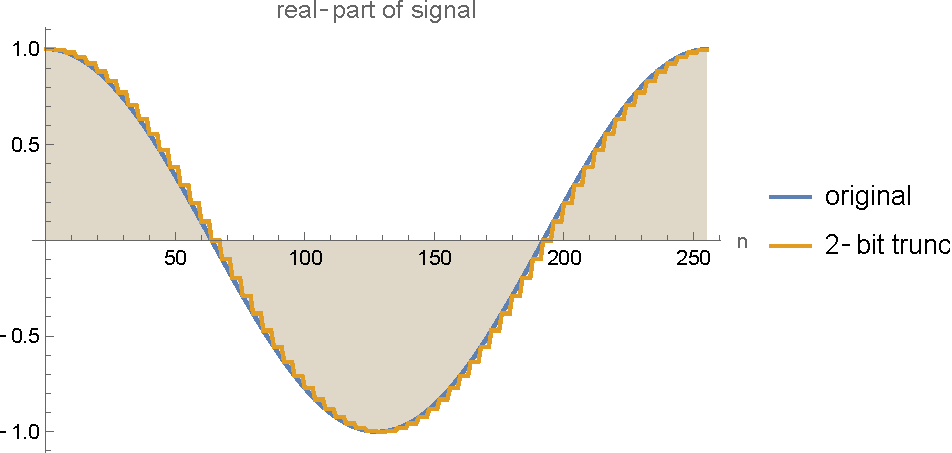
\includegraphics[keepaspectratio, scale=0.7]
                {\currfiledir/figs/real-part_of_NCO_output.pdf}
                \caption{NCO の出力の実部}
            \end{figure}
            \begin{figure}[H]
                \centering
                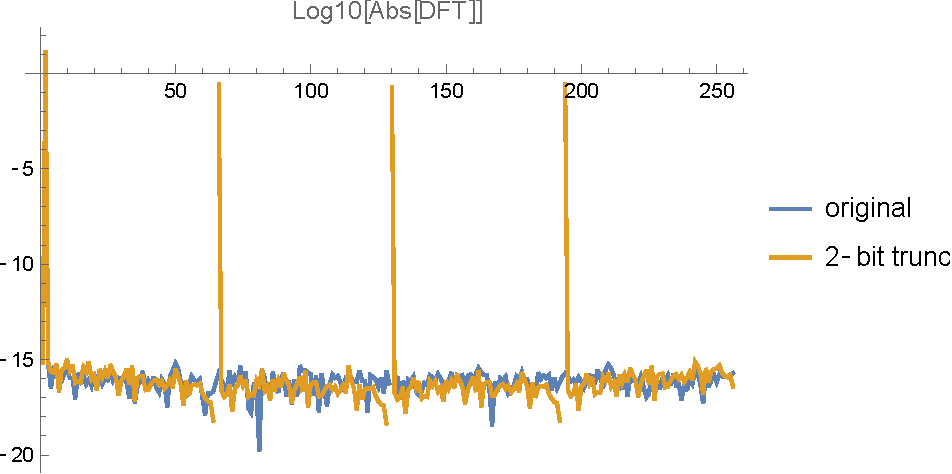
\includegraphics[keepaspectratio, scale=0.7]
                {\currfiledir/figs/Log10[Abs[DFT]].pdf}
                \caption{$\log_{10}X_W$}
            \end{figure}